\documentclass[11pt]{article}
% Build:  python paper/make_figures.py && cd paper && pdflatex main && bibtex main && pdflatex main && pdflatex main
% Rule (PAPER_PLAN.md): no number appears in this text unless runs/paper/<step>_RESULT.md (or, for the appendix,
% runs/<study>/RESULT.md) holds it. Everything else is \todo{}.

\usepackage[margin=1in]{geometry}
\usepackage[T1]{fontenc}
\usepackage[utf8]{inputenc}
\usepackage{lmodern}
\usepackage{amsmath,amssymb}
\usepackage{booktabs}
\usepackage{graphicx}
\usepackage{xcolor}
\usepackage[numbers,sort&compress]{natbib}
\usepackage[colorlinks=true,linkcolor=blue!50!black,citecolor=blue!50!black,urlcolor=blue!50!black]{hyperref}

\newcommand{\todo}[1]{\textcolor{red}{[TODO: #1]}}
\newcommand{\NS}{\operatorname{NS}}
\newcommand{\RTN}{\operatorname{RTN}}
\newcommand{\SR}{\operatorname{SR}}
\newcommand{\norm}[1]{\lVert #1 \rVert}

\title{Masterless Muon: Training 4-bit Weights Without a Full-Precision Copy}
\author{\todo{Author names and affiliations}}
\date{\todo{date}}

\begin{document}
\maketitle

% ======================================================================================================================
\begin{abstract}
Low-bit training normally keeps a full-precision copy of every weight: the optimizer updates the copy and the
low-bit weights are re-derived from it. Recent work removes the copy by feeding each step's rounding error back into
the optimizer's momentum. We show that this fails for Muon, and explain why: Muon orthogonalises its momentum, so its
update has a nearly fixed size, and an error fed into the momentum loses its size and much of its direction on the
way through the Newton--Schulz iteration (on pretrained GPT-2 the delivered correction keeps a cosine of only
0.65--0.77 with the intended one, and at the size ECO's rule calls for, under 5\% of it arrives). We propose the \emph{ticker}: the weights are stored only on a 4-bit grid (E2M1,
one scale per 16 weights), and a per-weight carry of $b$ bits, measured in units of that weight's own grid gap, holds
the part of each step that has not yet moved the weight. With an 8-bit carry and 8-bit momentum the training state is
about 2.8 bytes per weight, and the weights being trained \emph{are} the 4-bit weights that are served. On GPT-2
small (124M, continued training on 100M tokens) the ticker ends 0.0013 from training with an 8-byte float copy and
0.0012 from an exact fp32 carry, and 0.043--0.049 below bf16 weights with stochastic rounding once both are rounded to
4 bits. Trained from scratch (45M, 0.9B tokens) it ends within 0.013 of the float copy on every seed, while a bf16
model rounded to 4 bits afterwards loses 1.16. A noise model for the carry fails its own tests; an 8-bit carry was
enough at every learning rate we tried. In full-parameter reinforcement learning of Qwen3.5-0.8B on GSM8K with every
decoder weight in 4 bits and no float copy, the model gains 20.4 points over its 4-bit start, and the trainer and the
answer generator use the same 4-bit weights. It ends 3.7 points behind full-precision training (95\% interval $-5.2$ to $-2.2$), failing our pre-registered line of $-4$; most of that gap is the 6.5 points lost by rounding the model to 4 bits before training. A frozen 4-bit model with a 16-bit LoRA add-on ends 2.6 points above ours, but its gain lives entirely in the add-on: merged and rounded to 4 bits, not one weight changes and it scores its 4-bit start, 20.9 points below ours. With real packed storage a
full-parameter training step peaks at 0.32 of the standard bf16-plus-fp32-copy setup.
\end{abstract}

% ======================================================================================================================
\section{Introduction}

Training a model whose weights are 4-bit numbers almost always means training a different, full-precision model.
The standard recipe keeps an fp32 (or bf16) \emph{master copy} of each weight; the optimizer adds its small update
to the copy, and the 4-bit weights used in the forward pass are re-rounded from it at every step. The copy is needed
because a single step is usually far smaller than the distance between neighbouring 4-bit values: rounded on its own,
the step would vanish. The cost is that the model being trained is not the model being served. In reinforcement
learning (RL) this shows up directly: the 4-bit generator that writes answers and the full-precision trainer that
scores them are different weights, and the mismatch has to be corrected for \citep{yao2025offpolicy,liu2025flashrl}.

\paragraph{One sentence.} Muon breaks error feedback, and a quantized carry measured in units of each weight's own
grid gap fixes it. So the weights you train \emph{are} the 4-bit weights: the trained model and the model that writes
RL answers are the same weights, with no float copy.

\paragraph{Error feedback and why it does not carry over to Muon.} ECO \citep{nikdan2026eco} removes the master copy
for SGD with momentum and for Adam: after each step, the rounding error is added into the momentum, scaled so that
the optimizer re-applies it over the following steps. This works because both optimizers are \emph{linear} in the
momentum (Adam is linear once its second moment is fixed), so an error put into the momentum comes out in the weights
unchanged. Muon \citep{jordan2024muon,liu2025moonlight} is not linear in its momentum. It replaces the momentum by an
approximately orthogonal matrix with the same singular vectors (Newton--Schulz iteration), so its update has a nearly
fixed size whatever the momentum's size. We show, with a measurement on pretrained GPT-2 that needs no training
(Section~\ref{sec:mechanism}), that an error fed into Muon's momentum loses its size and part of its direction on the
way to the weights.

\paragraph{The ticker.} Instead of routing the error through the optimizer, we keep it beside each weight. Each weight
stores a 4-bit value and a small integer \emph{carry}: the part of the weight's intended position that the 4-bit grid
cannot show yet, in units of the gap to the next grid value on that side. Each step adds the update to weight plus
carry, rounds to the nearest grid value, and keeps the rest as the new carry, rounded at random to $b$ bits. With an
exact (fp32) carry this is Kahan's compensated summation \citep{kahan1965} on 4-bit weights, and it is mathematically
the same as training with a float copy. The question is how few bits the carry can have.

\paragraph{Contributions.}
\begin{enumerate}
  \item \textbf{The mechanism.} Muon's orthogonalised update has a nearly fixed size, so (i) an error fed into its
        momentum does not reach the weights intact, which is why ECO fails with Muon, and (ii) the per-step travel of
        each weight is predictable, which makes a noise model for low-bit carries simple
        (Section~\ref{sec:mechanism}).
  \item \textbf{The ticker}: 4-bit weights, an 8-bit carry in units of the weight's own gap, and 8-bit momentum,
        about 2.6--2.8 bytes per weight (Section~\ref{sec:method}). It is within 0.0013 (continued training of GPT-2
        small) and 0.013 (45M from scratch) of training with a float copy, within 0.0012 of an exact fp32 carry, and
        beats bf16 weights with random rounding once both are rounded to 4 bits, by 0.04--0.05 and by 1.13.
  \item \textbf{A noise model} for the smallest carry that works at a given learning rate
        (Section~\ref{sec:noise}). It \emph{fails} its pre-registered tests on a grid of 4 carry widths and 4
        learning rates; the damage depends on the carry width, not the learning rate, and 8 bits was always enough.
  \item \textbf{Full-parameter RL on 4-bit weights} with one copy of the weights: Qwen3.5-0.8B gains 20.4 points on
        GSM8K, with the generator and the trainer on the same 4-bit weights. It fails its pre-registered line against full-precision training ($-3.7$, interval $[-5.2, -2.2]$, line $-4$). Served with its 16-bit add-on, LoRA ends 2.6 points above ours; as a pure 4-bit model it keeps none of its gain, and ours is 20.9 points above it.
  \item \textbf{Memory, measured}, against the strongest baseline we know (bf16 weights with random rounding), which
        ours beats by only 5--13\% (0.87--0.95 of its peak); against the standard setup it is 0.32. The pitch of this paper is native 4-bit weights,
        not memory.
\end{enumerate}

% ======================================================================================================================
\section{Method}\label{sec:method}

\subsection{The 4-bit format}
Each weight matrix $W\in\mathbb{R}^{m\times n}$ (output $\times$ input) is split into blocks of 16 consecutive weights
along the input dimension. A block has one scale $s = \max_i |w_i| / 6$, and each weight is $w = s\,x$ with $x$ from
the signed E2M1 value set
\[
  x \in \{0, \pm 0.5, \pm 1, \pm 1.5, \pm 2, \pm 3, \pm 4, \pm 6\},
\]
as in NVFP4 \citep{nvidia2025nvfp4} (MXFP4 \citep{rouhani2023mx} uses the same values with a power-of-two scale per
32 weights). $\RTN(\cdot)$ rounds to the nearest grid value. For a grid value $x$ we write $g_+(x)$ and $g_-(x)$ for
the gaps to the next value up and down (0.5, 1 or 2 times $s$; beyond $\pm 6$ we use 2). In our experiments the
scale is kept in fp32; NVFP4 stores it in FP8 (E4M3) with one fp32 scale per tensor, which saves 0.19 bytes per
weight. Only the matrices inside the transformer blocks are stored this way and trained by Muon; embeddings, norms
and biases stay in floating point and are trained by AdamW, as is usual for Muon.

\subsection{The ticker}
Let $\hat w$ be a weight's stored 4-bit value, $c$ its carry, $\eta$ the learning rate and $\Delta$ the optimizer's
update for this step. One step is
\begin{align}
  \tilde w &= \hat w + c - \eta \Delta && \text{(where the weight should be)} \label{eq:target}\\
  \hat w' &= \RTN(\tilde w) && \text{(nearest 4-bit value; block scale recomputed)}\\
  r &= \tilde w - \hat w' && \text{(what the grid cannot show yet)}\\
  k' &= \SR\!\left(2L \, \frac{r}{g_{\pm}(\hat w')}\right) \in \{-L,\dots,L\} && \text{(the new carry, as an integer)}\\
  c' &= \frac{k'}{2L}\, g_{\pm}(\hat w') && \text{(the value it stands for)}
\end{align}
where $g_\pm$ is the gap on the side of $r$'s sign, $L = 2^{b-1}-1$ for a $b$-bit carry, and $\SR$ rounds to one of
the two neighbouring integers at random, with probabilities that make it unbiased. Because $\hat w'$ is the
\emph{nearest} grid value, $|r| \le g_\pm/2$, so $|k'| \le L$ and the carry never clips. A weight ``ticks'' to the next
grid value when its carry passes half a gap. The carry is relative to the weight's own gap, so a small weight (fine
gaps) and a large weight (coarse gaps) both get $2L$ levels of resolution. At $b=8$ the resolution is $1/254$ of a gap.

\paragraph{Relation to compensated summation.} With $c$ kept exactly in fp32, $\hat w + c$ equals the float-copy
weight at every step, given the same updates: the method is Kahan summation \citep{kahan1965} with a 4-bit main term.
The ticker quantizes the compensation term, in units that follow the main term's local resolution. Its only error
relative to a float copy is the random rounding of the carry (and of the momentum); Section~\ref{sec:noise} sizes it.
Error Diffusion \citep{bonin2026errordiffusion} uses the same idea for binary weights: a few-bit residual buffer per
weight, updated with stochastic rounding, that flips the weight when it crosses a threshold. The ticker is the
multi-level form of that buffer (Section~\ref{sec:related}).

\subsection{8-bit momentum}
Muon's momentum is stored as 8-bit integers ($-127\dots127$) with one fp32 scale per 128 weights of a row, rounded at
random after each update. Newton--Schulz runs on the dequantized Nesterov momentum.

\subsection{Bytes per weight}
Table~\ref{tab:bytes} counts the training state of the block matrices (weights plus optimizer state; gradients and
activations are the same for all methods and not counted).

\begin{table}[t]
\centering
\caption{Training state per weight of the Muon-trained matrices. Scales: one fp32 scale per 16 weights (0.25 bytes per
weight) or, in brackets, NVFP4-style FP8 scales (0.0625). Momentum scale: one fp32 scale per 128 (0.03).}
\label{tab:bytes}
\small
\begin{tabular}{lll}
\toprule
method & parts & bytes/weight \\
\midrule
4-bit + float copy, AdamW & fp32 copy + two fp32 moments & 12 \\
4-bit + float copy, Muon & fp32 copy + fp32 momentum & 8 \\
Kahan (exact carry) & 4-bit + scale + fp32 carry + 8-bit mom. & 5.78 \\
bf16-SR & bf16 weight + 8-bit momentum & 3.03 \\
\textbf{ours, 8-bit carry} & 4-bit + scale + 8-bit carry + 8-bit mom. & \textbf{2.78} (2.59) \\
naive / ECO-Muon & 4-bit + scale + 8-bit mom. & 1.78 (1.59) \\
\bottomrule
\end{tabular}
\end{table}

% ======================================================================================================================
\section{The mechanism: Muon's update has a fixed size}\label{sec:mechanism}

\subsection{Muon}
For a matrix $W$ with gradient $G_t$, Muon \citep{jordan2024muon} keeps a momentum $B_t = \beta B_{t-1} + (1-\beta) G_t$
and orthogonalises the Nesterov combination $U_t = (1-\beta)G_t + \beta B_t$:
\[
  W \leftarrow W - \eta\, \alpha\, \NS(U_t), \qquad \alpha = \sqrt{\max(1, m/n)} ,
\]
where $\NS$ is five steps of a quintic Newton--Schulz iteration, $X \leftarrow aX + (bA + cA^2)X$ with $A = XX^\top$,
$(a,b,c) = (3.4445, -4.7750, 2.0315)$, started from $X = U/\norm{U}_F$. If $U = P\Sigma Q^\top$ is a singular value
decomposition, $\NS(U) = P f(\Sigma/\norm{U}_F) Q^\top$ for a fixed odd polynomial $f$ that maps every singular value
that is not tiny into roughly $[0.7, 1.2]$. Two facts follow.

\paragraph{Fact 1: the step size is nearly fixed.} $\NS(cU) = \NS(U)$ for every $c>0$, and
$\norm{\NS(U)}_F \approx \bar f \sqrt{\min(m,n)}$ with $\bar f$ the root-mean-square of $f$ over the singular values.
So each step moves the matrix by $\eta\alpha\bar f\sqrt{\min(m,n)}$ in Frobenius norm, or
$\eta\alpha\bar f/\sqrt{\max(m,n)}$ per weight (root-mean-square), whatever the size of the gradient. On GPT-2 we
measure $\bar f = 0.905$ (standard deviation 0.066, range 0.69--0.99) over 48 matrices and 40 steps, while the
momentum's own RMS varies by a factor of 49 (Figure~\ref{fig:m}c); multiplying the momentum by $10^{3}$ or $10^{-3}$
changes the update by less than 0.02\%.

\paragraph{Fact 2: an error added to the momentum does not pass through.} ECO \citep{nikdan2026eco} adds
$\alpha_{\text{ECO}}\, e$ to the momentum, with $e$ the rounding error of the last step and
$\alpha_{\text{ECO}} = \eta^{-1}(1-\beta^{-1})$ for SGD with momentum (and the same times Adam's per-weight step size for
Adam). For an optimizer whose update is a linear function of the momentum, this puts exactly $(1-\beta)e$ into the next
step and $e$ into the sum of all later steps, so the weight ends up where the float copy would have put it. Muon's
update is not linear in the momentum. To first order, for a small error $\delta$ added to $U$ (take $m \le n$), the
change in the exact orthogonal factor $PQ^\top$ is
\begin{equation}\label{eq:polar}
  d(PQ^\top) = P\, K\, Q^\top + P\,\Sigma^{-1} P^\top \delta\,(I - QQ^\top), \qquad
  K_{ij} = \frac{\tilde\delta_{ij} - \tilde\delta_{ji}}{\sigma_i + \sigma_j}, \quad \tilde\delta = P^\top \delta Q .
\end{equation}
Compared with passing $\delta$ through at the update's average gain $\kappa = \norm{\NS(U)}_F/\norm{U}_F$, three
things happen:
\begin{enumerate}
  \item \textbf{The symmetric part of $\tilde\delta$ is discarded.} It only changes the singular values, and
        orthogonalisation sets them all to about 1. On GPT-2 this is 22\% of the energy of the actual 4-bit rounding
        error (7--50\% by matrix).
  \item \textbf{The rest is reweighted by $\sigma_{\text{rms}}/\sigma_i$.} Directions with small singular values are
        amplified and the few large ones, where the gradient's signal lives, are damped. Momentum spectra are
        heavy-tailed, so the delivered correction points somewhere else than the error. Newton--Schulz caps the
        amplification: its slope at zero is $a^5 \approx 485$ on the normalised input, which is at most about
        $485/(\bar f\sqrt{\min(m,n)}) \approx 19$ times $\kappa$ for GPT-2's $768$-wide matrices.
  \item \textbf{Large errors saturate.} By scale invariance $\NS(U+\delta) \to \NS(\delta)$ as
        $\norm{\delta}/\norm{U} \to \infty$, so $\norm{\NS(U+\delta) - \NS(U)}_F \le 2\bar f\sqrt{\min(m,n)}$: the
        delivered change is bounded, and the share of the intended correction that arrives falls like
        $\norm{U}/\norm{\delta}$.
\end{enumerate}
No choice of the injection scale fixes this: a small injection is bent and amplified, a large one is bent and
truncated, and in between the gradient's own direction is overwritten.

\subsection{Measurement on GPT-2 (no training)}\label{sec:m}
We take pretrained GPT-2 small \citep{radford2019gpt2}, compute real gradients of its 48 block matrices on FineWeb windows, and build Muon's
Nesterov momentum over 40 steps (2 windows of 1,024 tokens each). We then add into $U$ an error whose
direction is each matrix's actual 4-bit rounding leftover $W - \RTN(W)$, at sizes from 0.01 to 10 times $\norm{U}$,
and compare the change in the update with the error (Figure~\ref{fig:m}, Table~\ref{tab:m}). For SGD with momentum
the error passes through exactly. Adam with ECO's per-weight rule also passes it through exactly, because ECO
multiplies the error by the same per-weight factor that Adam divides by; injected without that factor, Adam rescales
it weight by weight (cosine 0.80). For Muon, the cosine between the delivered and the intended
correction is 0.65--0.77 at every size (single matrices 0.48--0.91), and the share of the intended correction that
arrives along the error falls from 7.6 at size 0.01 (small errors are amplified) through 0.90 at size 1 to 0.093 at
size 10. At the size ECO's rule gives for this error at learning rate $10^{-3}$ (22 times the momentum on average),
4.6\% of the intended correction arrives, and the update keeps a cosine of only 0.015 with the error-free update: the
gradient's direction is gone. Even an error one tenth the size of the momentum turns the update by about $40^\circ$
(cosine 0.76 with the error-free update). A random error direction behaves the same way, so this is a
property of Newton--Schulz, not of the 4-bit leftover. An earlier training-time measurement on a small character-level
model found the same cosine, about 0.69, and showed ECO-Muon training ending worse than no error feedback at all
(Appendix~\ref{app:toy}).

\begin{figure}[t]
\centering
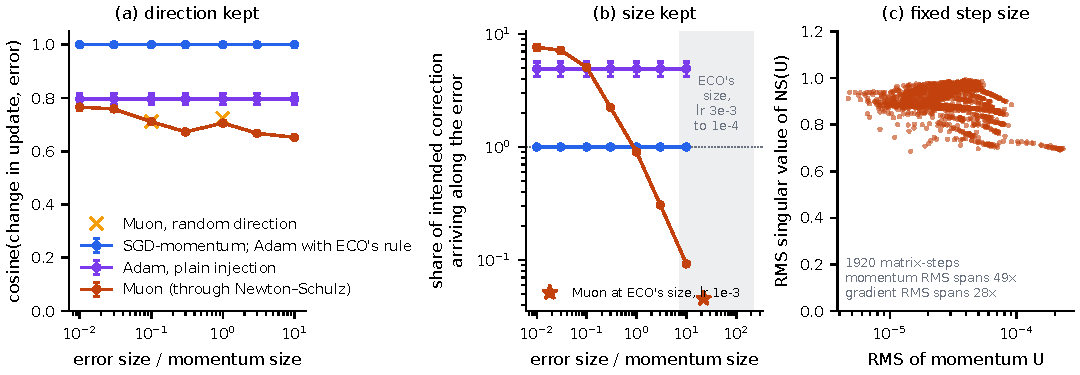
\includegraphics[width=\linewidth]{figures/m_ns_survival.pdf}
\caption{Error fed into the momentum, pretrained GPT-2 small, 48 block matrices (mean $\pm$ standard error over
matrices). (a) Cosine between the change in the update and the injected error. (b) Share of the intended correction
that arrives along the error ($=$ cosine $\times$ size ratio; 1 means it passes through intact); the grey band is the
size ECO's rule gives at learning rates $3\cdot10^{-3}$ to $10^{-4}$. (c) Muon's step size: the RMS singular value of
$\NS(U)$ against the RMS of the momentum $U$, for every matrix and step.}
\label{fig:m}
\end{figure}

\begin{table}[t]
\centering
\caption{Survival of an error added to the momentum (actual 4-bit rounding leftover as direction). Mean over the 48
block matrices of GPT-2 small, momentum built over 40 steps (\texttt{runs/paper/M\_RESULT.md}). Share arriving: the
part of the change along the error, as a share of the error passed through at the optimizer's average gain.}
\label{tab:m}
\begin{tabular}{lccc}
\toprule
optimizer & cosine & size ratio & share arriving along the error \\
\midrule
SGD-momentum & 1 & 1 & 1 \\
Adam, ECO's rule & 1 & 1 & 1 \\
Adam, plain injection & 0.80 & 7.3 & 4.9 \\
Muon, error $=0.1\times$ momentum & 0.71 & 7.1 & 5.1 \\
Muon, error $=1\times$ momentum & 0.71 & 1.28 & 0.90 \\
Muon, error $=10\times$ momentum & 0.65 & 0.142 & 0.093 \\
Muon, ECO's size at $\eta = 10^{-3}$ ($22\times$) & 0.65 & 0.071 & 0.046 \\
\bottomrule
\end{tabular}
\end{table}

% ======================================================================================================================
\section{A noise model for the carry}\label{sec:noise}

The ticker differs from a float copy only through random rounding of the carry (and of the momentum, which we leave
out here). Each step rounds the carry to a multiple of $u_b = g/(2L) \approx g/2^b$, where $g$ is the weight's gap.
Stochastic rounding is unbiased, and its error on one step has variance $p(1-p)u_b^2 \le u_b^2/4$. Fresh random bits
are drawn at every step, so the errors are independent and after $T$ steps they add up to a random drift of standard
deviation at most
\[
  D_b(T) = \frac{u_b}{2}\sqrt{T} \approx \frac{g}{2^b}\cdot\frac{\sqrt{T}}{2} .
\]
Meanwhile Muon moves each weight by about $\eta\, \alpha\bar f/\sqrt{\max(m,n)} =: \eta\, \bar u$ per step (Fact 1).
If the weight keeps moving in one direction its intended travel is $\eta\bar u T$, and the ratio
\[
  \rho = \frac{D_b(T)}{\eta\,\bar u\,T} = \frac{g}{2^{b+1}\,\eta\,\bar u\,\sqrt{T}}
\]
measures how much of that travel is noise. A carry of $b$ bits is enough when $\rho$ is below a threshold $\rho^*$,
which we fit on two learning rates and test on two others (Section~\ref{sec:p3}).

\paragraph{Assumptions, stated honestly.}
(i) Rounding errors at different steps are independent; this holds for the random bits, but the weight's position
also feeds back into the gradient. (ii) Travel is linear in $T$. If the update's sign flips from step to step, the
travel grows more slowly (like $\sqrt{T}$ for a pure random walk), and $\rho$ underestimates the damage. (iii) The gap
$g$ is fixed; in reality it changes when a weight moves to another grid cell or the block's largest weight changes the
scale. (iv) The momentum's 8-bit rounding noise is ignored. (v) The model predicts a per-weight noise level, not the
loss: mapping $\rho$ to a loss gap assumes the damage grows with $\rho$ (P3a tests only the ranking). The model is
cleaner for Muon than for Adam because Fact 1 makes $\bar u$ a constant of the matrix shape; under Adam the per-weight
step $|\hat m|/\sqrt{\hat v}$ varies with each weight's gradient signal-to-noise ratio.

% ======================================================================================================================
\section{Experiments}\label{sec:experiments}

All pass lines were written before the runs (\texttt{PAPER\_PLAN.md}, revision 3) and are reported whether or not
they hold. Within a table all arms run on the same GPU type and number format. Seeds: 3 for close arms, 1 for arms
expected to be far apart; a 1-seed gap counts only if it exceeds 10 times the largest seed standard deviation of the
same table. Every loss carries a paired standard error over 256 fixed validation windows of 1,024 tokens.

\subsection{P1: GPT-2 small, continued training (headline)}\label{sec:p1}
Pretrained GPT-2 small \citep{radford2019gpt2}, 100M FineWeb \citep{penedo2024fineweb} tokens (3,050 steps of
$32\times1024$ tokens), Muon at $10^{-3}$ on the 48 block matrices and AdamW at $10^{-4}$ on the rest, 5\% warm-up
then cosine to 10\%. One A100, fp16 with loss scaling, TF32 off, deterministic. Arms: ours (8-bit carry, 8-bit
momentum), 4-bit with a float copy and Muon, bf16 weights with random rounding and 8-bit momentum (bf16-SR), Kahan
(ours with an exact fp32 carry), float Muon, 4-bit with a float copy and AdamW, naive (4-bit weights rounded at random,
no carry) and ECO-Muon (ECO's injection into Muon's momentum). Table~\ref{tab:p1} gives the final losses; all four pass
lines hold.

\begin{table}[t]
\centering
\caption{P1: final validation loss, GPT-2 small, 100M tokens. $\pm$: paired standard error over 256 windows
(evaluation noise). Seed standard deviation (largest 3-seed arm) 0.0033, so a 1-seed gap counts only above 0.033.}
\label{tab:p1}
\small
\begin{tabular}{lcccc}
\toprule
arm & bytes/weight & seed 1 & seed 2 & seed 3 \\
\midrule
\textbf{ours} & 2.78 & 3.2884 & 3.2892 & 3.2889 \\
4-bit + float copy, Muon & 8 & 3.2873 & 3.2886 & 3.2866 \\
bf16-SR, rounded to 4 bits & 3.03 & 3.3346 & 3.3387 & 3.3322 \\
bf16-SR, scored in bf16 & 3.03 & 3.2690 & 3.2720 & 3.2695 \\
Kahan (fp32 carry) & 5.78 & 3.2872 & & \\
float Muon & 8 & 3.2670 & & \\
float Muon, rounded to 4 bits & 8 & 3.3303 & & \\
4-bit + float copy, AdamW & 12 & 3.2840 & & \\
naive (random rounding, no carry) & 1.78 & 3.4483 & & \\
ECO-Muon (Newton--Schulz in fp32) & 1.78 & 3.3253 & & \\
start: pretrained, rounded to 4 bits & & 3.4025 & & \\
\midrule
\multicolumn{5}{l}{P1a: ours $-$ float copy $= +0.0011, +0.0006, +0.0023$ ($\pm 0.0005$); line $+0.03$ \hfill PASS}\\
\multicolumn{5}{l}{P1b: naive $-$ ours $= 0.160$, ECO-Muon $-$ ours $= 0.037$ ($\pm 0.002$); line $0.02$ and $0.033$ \hfill PASS}\\
\multicolumn{5}{l}{P1c: bf16-SR rounded $-$ ours $= 0.046, 0.049, 0.043$ ($\pm 0.001$) \hfill PASS}\\
\multicolumn{5}{l}{P1d: ours $-$ Kahan $= +0.0012 \pm 0.0005$; line $0.01$ \hfill PASS}\\
\bottomrule
\end{tabular}
\end{table}

\begin{figure}[t]
\centering
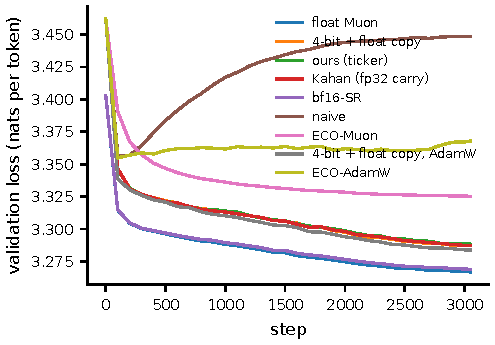
\includegraphics[width=0.48\linewidth]{figures/p1_curves.pdf}
\caption{P1: validation loss of every arm, seed 1. Ours, Kahan and the 4-bit float copy overlap; naive rounding gets
worse after the first steps; ECO-Muon stalls.}
\label{fig:p1}
\end{figure}

\paragraph{What it shows.} With 2.78 bytes per weight, ours ends 0.0013 (mean of 3 seeds) behind training the same
4-bit model with an 8-byte float copy, and 0.0012 behind an exact fp32 carry, so the 8-bit carry loses almost nothing.
Training in 4 bits beats training in higher precision and rounding at the end: bf16-SR is the best model while it is
scored in bf16, but rounded to 4 bits it is 0.043--0.049 worse than ours, and float Muon rounded to 4 bits is 0.042
worse. The price of 4-bit weights themselves (ours against float Muon in fp32) is $+0.021$, the same as for the float
copy ($+0.020$). ECO-Muon does better than naive rounding but freezes the 4-bit weights: only 0.0004\% of them change
per step (ours: 0.14\%), falling to zero by the end. The injected error dominates the momentum, so each step mostly
points back towards undoing the last rounding (Section~\ref{sec:mechanism}). Its first run, with Newton--Schulz in
fp16 like every other arm, overflowed by step 10, because the injected error makes the momentum far larger than usual;
the run in Table~\ref{tab:p1} repeats it with Newton--Schulz in fp32, which can only help it.

\subsection{P2: from scratch, 45M parameters}\label{sec:p2}
A GPT-2-style model with 6 layers of width 512 (45.2M parameters) is trained from random weights on 0.9B FineWeb
tokens (27,466 steps of $32\times1024$, about 20 tokens per parameter). The Muon learning rate (0.04, with AdamW at
$4\cdot10^{-3}$) was picked from three by short runs of the float copy, the same rate for every arm. Ours and the 4-bit
float copy run 3 seeds, bf16-SR one.

\begin{table}[t]
\centering
\caption{P2: final validation loss, 45M model from scratch, 0.9B tokens.}
\label{tab:p2}
\small
\begin{tabular}{lccccc}
\toprule
arm & bytes/weight & seed 1 & seed 2 & seed 3 & mean $\pm$ seed s.d. \\
\midrule
\textbf{ours} & 2.78 & 3.9127 & 3.9262 & 3.9196 & $3.9195 \pm 0.0067$ \\
4-bit + float copy, Muon & 8 & 3.9078 & 3.9133 & 3.9095 & $3.9102 \pm 0.0028$ \\
bf16-SR, scored in bf16 & 3.03 & 3.8894 & & & \\
bf16-SR, rounded to 4 bits & 3.03 & 5.0515 & & & \\
\midrule
\multicolumn{6}{l}{P2a: ours $-$ float copy $= +0.0049, +0.0128, +0.0101$ ($\pm 0.0019$); line $+0.03$ \hfill PASS}\\
\multicolumn{6}{l}{P2c: bf16-SR rounded $-$ ours $= 1.132$; line $2\times 0.0067$ \hfill PASS}\\
\bottomrule
\end{tabular}
\end{table}

\begin{figure}[t]
\centering
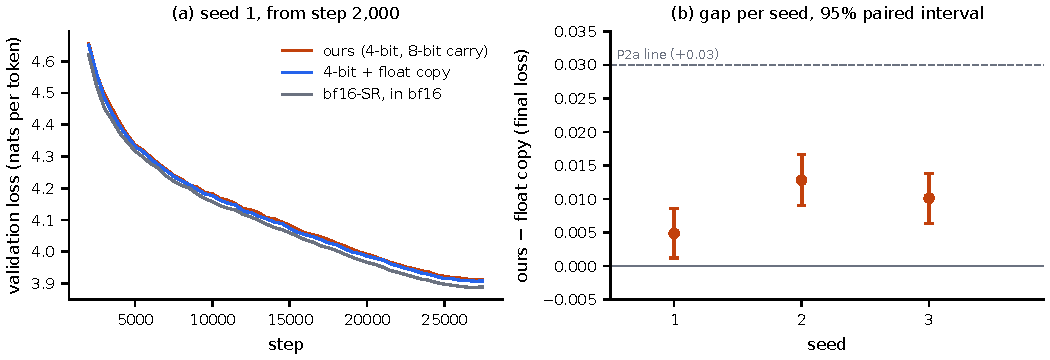
\includegraphics[width=\linewidth]{figures/p2_curves.pdf}
\caption{P2: (a) validation loss from step 2,000, seed 1; (b) ours minus the float copy at the end, per seed.}
\label{fig:p2}
\end{figure}

\paragraph{What it shows.} From scratch the gap to the float copy is larger than in continued training (mean
$+0.009$ against $+0.0013$) and resolved on every seed, but well inside the line, and the carry never overflowed.
Ours also varies more from seed to seed (0.0067 against 0.0028): the random rounding of the carry adds a little
seed noise. Training in 16 bits and rounding at the end does not survive from scratch at all: bf16-SR is the best model
in bf16 (3.889) and loses 1.16 when rounded to 4 bits. The chosen learning rate is the top of its grid, so a larger
one might be better for every arm.

\subsection{P3: the noise model}\label{sec:p3}
Continued training of GPT-2 small for 10M tokens (305 steps, same schedule shape), at Muon learning rates
$\{10^{-4}, 3\cdot10^{-4}, 10^{-3}, 3\cdot10^{-3}\}$, with carries of $\{4,6,8,12\}$ bits and the float copy at each
rate (20 runs, seed 1). Table~\ref{tab:p3} gives each cell's gap to the float copy and Figure~\ref{fig:p3} plots it
against $\rho$. \textbf{Both pass lines fail.} The rank correlation between $\rho$ and the gap is 0.795 (P3a, line
0.8). The threshold fitted on the two middle rates, $\rho^* = 1.01$, separates working from failing cells there without
error, but on the held-out rates it predicts 12 bits at $10^{-4}$, where 6 bits already worked (P3b: two levels off).

\begin{table}[t]
\centering
\caption{P3: ours minus the float copy at the same learning rate, 10M tokens, seed 1 ($\pm$: paired standard error).}
\label{tab:p3}
\small
\begin{tabular}{lcccc}
\toprule
carry bits & $10^{-4}$ & $3\cdot10^{-4}$ & $10^{-3}$ & $3\cdot10^{-3}$ \\
\midrule
4 & $+0.0425 \pm 0.0013$ & $+0.0518 \pm 0.0012$ & $+0.0513 \pm 0.0012$ & $+0.0452 \pm 0.0010$ \\
6 & $-0.0013 \pm 0.0004$ & $+0.0017 \pm 0.0005$ & $+0.0041 \pm 0.0005$ & $+0.0022 \pm 0.0006$ \\
8 & $-0.0005 \pm 0.0002$ & $-0.0002 \pm 0.0003$ & $-0.0000 \pm 0.0003$ & $-0.0006 \pm 0.0005$ \\
12 & $-0.0001 \pm 0.0001$ & $+0.0001 \pm 0.0002$ & $+0.0004 \pm 0.0003$ & $+0.0007 \pm 0.0005$ \\
\bottomrule
\end{tabular}
\end{table}

\begin{figure}[t]
\centering
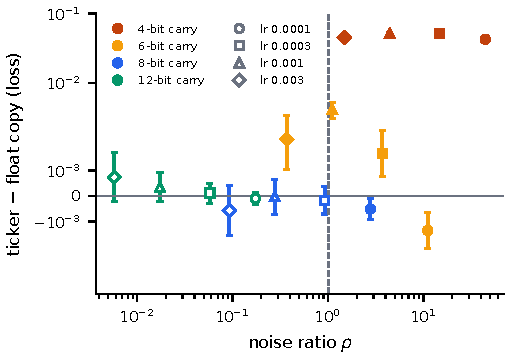
\includegraphics[width=0.5\linewidth]{figures/p3_noise_model.pdf}
\caption{P3: gap to the float copy against the noise ratio $\rho$ (bars: 2 paired standard errors; open markers:
within 2 errors of zero). Dashed: the fitted threshold $\rho^*$.}
\label{fig:p3}
\end{figure}

\paragraph{Why it fails, and what holds instead.} The damage depends on the carry width and hardly on the learning
rate: 4 bits costs about 0.045 at every rate, 6 bits 0.002--0.004, and 8 and 12 bits nothing measurable. The model
assumes each step adds a fixed amount of rounding noise, so small learning rates, which need many small steps, should
suffer most. They do not. Random rounding of a small change adds noise in proportion to that change (its variance is
about $u_b\,|\text{step}|$, not $u_b^2/4$), so the noise shrinks with the step. The carry width alone ranks the cells
with a correlation of 0.92; this is a reading after the data, not a tested claim. In practice an 8-bit carry was
enough at every learning rate we tried, and the RL experiments use it. Before any RL result, the failed model
predicted a 12-bit carry for P5; that prediction was recorded and not tested.

\subsection{P4: ablations}\label{sec:p4}
Starting from ours, one thing is changed at a time (GPT-2 small, 25M tokens, seed 1; looks, not pass lines).

\begin{table}[t]
\centering
\caption{P4: one change at a time (GPT-2 small, 25M tokens, seed 1).}
\label{tab:p4}
\small
\begin{tabular}{lccc}
\toprule
run & final loss & minus ours & changing per step \\
\midrule
ours & 3.3047 & & 0.133\% \\
carry in absolute units (block's largest gap) & 3.3059 & $+0.0012 \pm 0.0005$ & 0.101\% \\
weight rounded at random, not to nearest & 3.3759 & $+0.0713 \pm 0.0012$ & 31.2\% \\
Error Diffusion's cap (0.25 gap per step) & 3.3043 & $-0.0004 \pm 0.0004$ & 0.133\% \\
\bottomrule
\end{tabular}
\end{table}

Rounding the weight to nearest matters most: with random rounding a third of the weights flip every step and the
loss is 0.071 worse. Measuring the carry in units of each weight's own gap helps a little (0.0012). Error Diffusion's
per-step cap never binds at this learning rate, since Muon's steps are far below a quarter of a gap.

\subsection{P5: full-parameter RL in 4 bits}\label{sec:p5}
\paragraph{Setup.} Qwen3.5-0.8B (post-trained, non-thinking mode), GSM8K \citep{cobbe2021gsm8k}, GRPO
\citep{shao2024deepseekmath} with 8 answers to each of 32 questions per step, reward 1 if the final number is right,
200 steps, no KL term, one update per step. Answers are written by vLLM in the same process, with the trained
weights copied in (in bf16) after every step. The exam is the 1,319 test questions, greedy, at the start and the end.
Three arms:
(a) full-parameter training in bf16 with an fp32 copy, Muon on the decoder matrices;
(b) the 4-bit model frozen, with LoRA \citep{hu2022lora} of rank 32 on every decoder matrix, trained with AdamW at
$10^{-5}$ (QeRL-style \citep{huang2025qerl});
(c) ours: every decoder matrix stored in 4 bits with an 8-bit carry, Muon.
(b) and (c) start from the same round-to-nearest 4-bit model. Muon's learning rate was $10^{-4}$ with a guard written
in advance; the guard fired ((a)'s training reward peaked near step 35 and collapsed, and its exam score fell from
54.7\% to 36.6\%), so as written every run uses $4\cdot10^{-5}$.

\begin{table}[t]
\centering
\caption{P5: GSM8K test accuracy (\%), Qwen3.5-0.8B, 200 RL steps. Intervals: 95\%, each question's result
averaged over seeds and paired across arms.}
\label{tab:p5}
\small
\begin{tabular}{lcccc}
\toprule
arm & weights as scored & start & end (per seed) & gain \\
\midrule
(a) bf16 + fp32 copy & bf16 & 54.7 & 72.9, 71.1, 72.9 & $+17.6 \pm 2.4$ \\
(b) 4-bit frozen + LoRA & 4-bit + bf16 add-on & 48.1 & 70.6, 70.2, 72.8 & $+23.1 \pm 2.5$ \\
(b) merged, rounded to 4 bits & 4-bit & 48.1 & --, 47.6, 47.8 & $-0.4 \pm 2.0$ \\
\textbf{(c) ours} & \textbf{4-bit} & 48.1 & 69.7, 67.7, 68.4 & $+20.4 \pm 2.4$ \\
\midrule
\multicolumn{5}{l}{P5a: (c) $-$ (a) $= -3.7$, interval $[-5.2, -2.2]$; line: lower end above $-4$ \hfill FAIL}\\
\multicolumn{5}{l}{P5b: (c) gain $= +20.4$, interval $[+18.0, +22.9]$; line: $\ge 5$, above 0 \hfill PASS}\\
\multicolumn{5}{l}{measured: (c) $-$ (b) $= -2.6 \pm 1.6$; (c) $-$ (b) rounded to 4 bits $= +20.9 \pm 2.2$}\\
\multicolumn{5}{l}{measured: 4-bit start $-$ float start $= -6.5 \pm 2.8$}\\
\bottomrule
\end{tabular}
\end{table}

\begin{figure}[t]
\centering
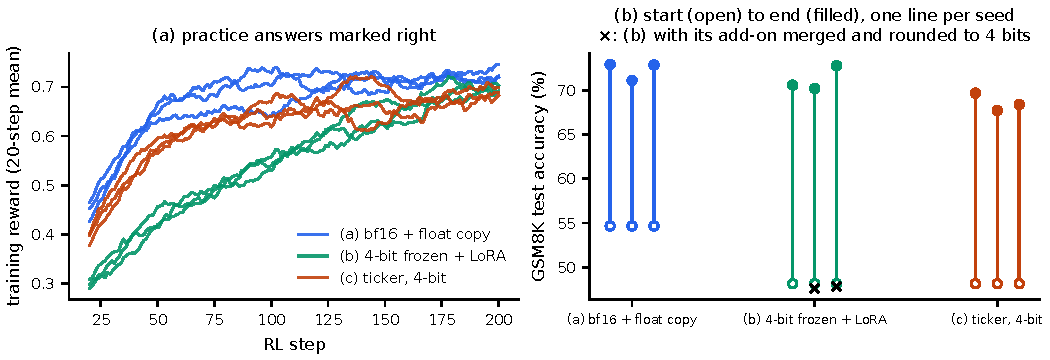
\includegraphics[width=\linewidth]{figures/p5_rl.pdf}
\caption{P5: (a) training reward, 20-step running mean, every run; (b) GSM8K test accuracy at the start and after 200
steps, one line per seed; $\times$: (b) with its add-on merged and rounded to 4 bits (seeds 2--3).}
\label{fig:p5}
\end{figure}

\paragraph{What it shows.} Every weight of the model learns while stored in 4 bits: ours gains 20.4 points, more
than full-precision training gains from its own start (17.6), and 0.11\% of the 4-bit values change per step. The
gap to (a) is the cost of the 4-bit start: rounding the model costs 6.5 points before any training, after 200 steps ours
is 3.7 behind, so it has closed about two fifths of it, not enough to pass P5a, and at 30 steps (a shorter design that was also run) ours had gained exactly as much as (a).
The generator and the trainer use the same 4-bit weights; the remaining gap between their token probabilities (mean
0.0033 for ours, 0.0030 for (a)) comes from the two programs' arithmetic, not from rounding. Against LoRA, ours learns
faster early (12 points ahead at 30 steps in the shorter design), and LoRA ends 2.6 points ahead after 200 steps
(interval $[-4.2, -1.0]$ for ours minus LoRA). The comparison is not like for like: (b) is scored with its add-on in
16 bits, as QLoRA-style methods are served, while ours is scored with 4-bit weights only. To measure what LoRA's gain
is worth as a 4-bit model, at the end of (b)'s seeds 2 and 3 we merged the add-on into the 4-bit weights and rounded
to the same grid, block scales recomputed. Before these runs we wrote down the prediction that most weights would
round back to their start and the model would score near its 48.1\% start. It held more strongly than written: the
add-on averages 0.5\% of the gap between neighbouring 4-bit values, \emph{no} 4-bit value changes, and the rounded
model scores 47.7\%, $23.8 \pm 2.3$ points below the same model with its add-on and $20.9 \pm 2.2$ below ours. LoRA's
gain is real but stored in 16 bits; ours is stored in the 4-bit weights themselves. Peak GPU memory in
these runs is set by the generator's reserved share and the activations (27--30 GB for (a) and (c), 24 GB for (b),
which needs no gradients or optimizer state for the frozen weights); the 4-bit values are held in fp32 tensors here,
so P6, not P5, measures the method's memory.

\subsection{P6: memory, measured}\label{sec:p6}
\texttt{p6\_memory.py} uses the release optimizer with real packed storage (two 4-bit codes per byte, FP8 block
scales, int8 carry, int8 momentum), applies the update to each matrix during the backward pass and frees its gradient
at once, and checkpoints activations. It measures one full-parameter training step of Qwen3.5-0.8B (752M parameters,
of which 498M in the decoder matrices) on a T4 with a batch of $2\times1024$ tokens.

\begin{table}[t]
\centering
\caption{P6: memory of one full-parameter training step of Qwen3.5-0.8B on a T4 (GiB).}
\label{tab:p6}
\small
\begin{tabular}{lccc}
\toprule
setup & peak & weights + state & peak / standard \\
\midrule
bf16 + AdamW with fp32 copy (standard) & 11.74 & 9.83 & 1.00 \\
float Muon & 10.33 & 6.56 & 0.88 \\
bf16-SR, 8-bit momentum & 4.31 & 2.40 & 0.37 \\
bf16-SR, updated layer by layer & 3.96 & 2.40 & 0.34 \\
\textbf{ours} & \textbf{3.74} & \textbf{2.18} & \textbf{0.318} \\
\bottomrule
\end{tabular}
\end{table}

\begin{figure}[t]
\centering
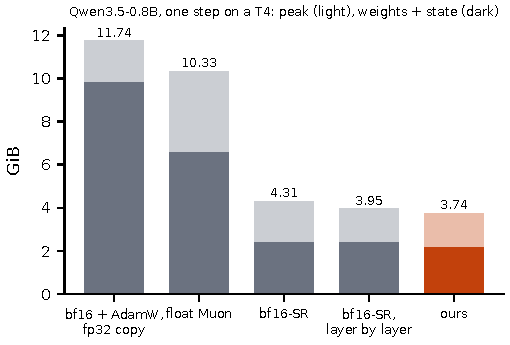
\includegraphics[width=0.5\linewidth]{figures/p6_memory.pdf}
\caption{P6: peak memory (light) and weights plus optimizer state (dark) of one training step.}
\label{fig:p6}
\end{figure}

Ours peaks at 0.318 of the standard setup (P6a, line 0.35: PASS). Against bf16-SR the saving is small: 0.87 of its
peak, 0.95 against bf16-SR with the same layer-by-layer update, and 0.91 in steady state. The decoder matrices alone
shrink by $2.59/3.03 = 0.86$, but the embedding is a third of this model and is stored the same way in both. The update
adds 4.8\,s to a 13.5\,s step in plain, unfused PyTorch. As a demonstration, a full-parameter step of Qwen3.5-2B fits
on the T4 at 8.34\,GiB in our format, where the standard setup runs out of memory.

% ======================================================================================================================
\section{Related work}\label{sec:related}

\paragraph{Training without master weights.} ECO \citep{nikdan2026eco} removes the master copy for SGD with momentum
and Adam by injecting the rounding error into the momentum; it proves exact equivalence to master weights for SGD with
momentum under an exact (memory-costly) rule and gives a noise-floor bound for the memory-free rule. We show why the
same injection fails for Muon (Section~\ref{sec:mechanism}). \emph{Error Diffusion} \citep{bonin2026errordiffusion},
which appeared days before this work, replaces the latent weight of a binary network with a 2--8-bit residual buffer
updated by stochastic rounding, flips a weight when the buffer crosses a threshold, and reports that the method works
best when the buffer grid has a level exactly at that threshold; it trains binary language models of up to about 19M
binary parameters. Our ticker is the multi-level form of that buffer: the threshold becomes half the gap to the
neighbouring 4-bit value on each side, and the buffer is measured in units of that gap. The parts that are new here
are Muon and the explanation of why error feedback through its momentum fails, 4-bit (E2M1) grids with per-block
scales, GPT-2-scale experiments, the noise model, and full-parameter RL. Bop \citep{helwegen2019bop} argued earlier
that binary networks need no latent weights at all and trains them with a momentum-threshold rule.

\paragraph{Compensated summation and stochastic rounding.} Kahan summation \citep{kahan1965} carries the low-order
part lost in each addition. \citet{zamirai2020bf16} show that pure bf16 training matches fp32 if weight updates use
stochastic rounding or Kahan summation, and Collage \citep{yu2024collage} represents weights as several low-precision
components to avoid fp32 copies. Stochastic rounding for deep learning goes back at least to
\citet{gupta2015limited}; \citet{croci2022sr} survey its theory and uses. Our bf16-SR baseline and our naive 4-bit
baseline are of this kind. The ticker differs by keeping the compensation term per weight, in few bits, and in units
of the main term's own local resolution.

\paragraph{Error feedback in compressed optimization.} Carrying a compression error forward to later steps is the
core of 1-bit SGD \citep{seide2014onebit} and of error-feedback methods for sign and compressed gradients
\citep{karimireddy2019efsgd}. There the error lives in the gradient communicated between machines; here it lives in
the weights.

\paragraph{Muon and low-bit Muon.} Muon \citep{jordan2024muon} orthogonalises the momentum of each matrix with a
Newton--Schulz iteration; \citet{liu2025moonlight} scale it to large language models. MuonQ \citep{su2026muonq} and
4-bit Muon with GRASP \citep{wu2026grasp} shrink Muon's \emph{optimizer state} to 4 bits, both noting that
orthogonalisation amplifies quantization error in the momentum (GRASP locates it in the top singular subspace); they
keep full-precision weights. Our measurement is the weight-side counterpart: error deliberately fed into the momentum
does not come out intact.

\paragraph{4-bit training.} NVFP4 \citep{nvidia2025nvfp4} and the microscaling formats \citep{rouhani2023mx} define the
4-bit values and block scales we use. Full-Stack FP4 \citep{ding2026fullstackfp4} pretrains with 4-bit projections,
optimizer states and attention but keeps bf16 master weights. FlashOptim \citep{gonzalezortiz2026flashoptim} reduces
optimizer memory and splits the master weight into lower-precision parts with a bound on the resulting error, so a
bf16-level master weight still exists.

\paragraph{RL with quantized weights.} QLoRA \citep{dettmers2023qlora} fine-tunes a frozen 4-bit model through a
16-bit low-rank add-on \citep{hu2022lora}; QeRL \citep{huang2025qerl} applies this to RL with an NVFP4 model, and our
arm (b) follows it. The trained model is then the 4-bit base plus a 16-bit add-on: QeRL's own evaluation attaches
the adapter to the NVFP4 model in vLLM, or merges it into a 16-bit model. Merging the add-on into the 4-bit weights
and rounding again can erase the adaptation, because the nearest grid point is usually the base itself;
Scale-QLoRA \citep{li2026scaleqlora} reports losses of up to 39 points and avoids them by training only the block
scales and freezing every 4-bit code. Ours goes the other way: every 4-bit code may change, and the trained model is
the 4-bit model, with no add-on to merge. In our LoRA arm the merge-and-round loss is total: no 4-bit value changes and the whole 23.8-point gain is lost (Section~\ref{sec:p5}).
FlashRL \citep{liu2025flashrl} generates rollouts with a quantized copy and corrects the
mismatch with the trainer by truncated importance sampling \citep{yao2025offpolicy}. With the ticker, the trainer and
the generator use the same 4-bit weights, so there is no rounding mismatch between them (other arithmetic differences
remain).

% ======================================================================================================================
\section{Limitations}\label{sec:limitations}
\begin{itemize}
  \item \textbf{Scale.} The largest training runs are GPT-2 small (124M, continued training) and a 45M model from
        scratch; RL uses Qwen3.5-0.8B. Behaviour at billions of parameters is not tested.
  \item \textbf{Memory.} Against bf16 weights with random rounding and 8-bit momentum, ours saves only 5--13\% at
        the peak. Against a frozen 4-bit model with LoRA it uses more training memory, since every weight needs a
        gradient and a carry. The case for the method is native 4-bit weights trained in full, not memory.
  \item \textbf{RL.} One model (0.8B), one task, 200 steps, three seeds. Ours ends 3.7 points behind bf16 training and
        fails its pre-registered line; whether the gap keeps closing with longer training, or with a short healing run
        before RL, is not tested. LoRA's learning rate was not tuned. The generator holds a bf16 copy of the 4-bit values.
  \item \textbf{Simulation.} Training runs keep the 4-bit values in fp32 tensors and do not pack codes; only P6
        measures real packed storage. Block scales are fp32 in training; FP8 scales are counted, not trained with
        (a small character-level test found them to cost little; Appendix~\ref{app:toy}).
  \item \textbf{The mechanism measurement} uses one model, one optimizer state built over a short window of steps,
        and one error direction (the rounding leftover of the pretrained weights) plus a random control; it does not
        follow the error through many steps of training.
  \item \textbf{The noise model} failed both of its tests (Section~\ref{sec:p3}); the alternative reading (noise in
        proportion to the step) was made after seeing the data and is not tested.
  \item \textbf{Only weights} are 4-bit. Activations and gradients stay in 16/32 bits; embeddings, norms and biases are
        not quantized.
\end{itemize}

% ======================================================================================================================
\bibliographystyle{plainnat}
\bibliography{refs}

\appendix
% ======================================================================================================================
\section{Earlier small-scale results}\label{app:toy}
These runs led to the method. They use a character-level GPT on Shakespeare (4 layers, width 128, 0.8M parameters,
2,000 steps; loss in nats per character, mean $\pm$ standard error over 3 seeds) and are not evidence for any main
claim. Numbers are from \texttt{runs/m1}--\texttt{m4}, \texttt{runs/m7}, \texttt{runs/ticker} and
\texttt{runs/twobit} (\texttt{RESULT.md} in each).

\paragraph{Muon breaks ECO (milestones 1--4, CPU).} Float Muon reached $1.6278 \pm 0.0032$ and AdamW
$1.9150 \pm 0.0034$. 4-bit weights with a float copy (Muon) reached $1.6463 \pm 0.0019$; without a copy, with random
rounding, $1.7636 \pm 0.0044$. ECO with Adam reached $1.9283 \pm 0.0039$, close to its own float AdamW, as the ECO paper
reports. ECO's injection adapted to Muon (error into the momentum before Newton--Schulz) reached $1.8981 \pm 0.0057$,
\emph{worse} than no feedback at all. Measured during training, the change Newton--Schulz made in response to the
injected error had a cosine of about 0.69 with the error (all steps, each of 3 seeds: 0.691, 0.692, 0.692), and the
error grew from 0.15 to 0.50 of the momentum's size as the learning rate decayed. Adding the error after
Newton--Schulz instead, from a 2-byte buffer, reached $1.6733 \pm 0.0043$.

\paragraph{The ticker (side study T, Colab T4, fp16).} With a 4-bit carry (2.28 bytes per weight) the ticker reached
$1.6501 \pm 0.0045$, against $1.6458 \pm 0.0035$ for 4-bit with a float copy (8 bytes), and beat a 4-bit buffer with
random rounding of the weight ($1.7120 \pm 0.0019$) and FP8 training rounded to 4 bits afterwards
($1.6717 \pm 0.0043$) in every seed.

\paragraph{2-bit weights (side study 2B).} With 2-bit weights an 8-bit carry reached $1.7476 \pm 0.0059$ against
$1.7253 \pm 0.0015$ for a float copy with Muon; a 4-bit carry reached $1.8027 \pm 0.0040$.

\paragraph{A first GPT-2 run with a 4-bit carry (side study G, seed 1, T4, fp16).} Continued training of GPT-2 small
for 100M tokens with a 4-bit carry ended $+0.0465 \pm 0.0010$ above 4-bit with a float copy, missing a 0.03 line. The
cause was a flaw of the 4-bit carry: after a tick the leftover is about half a gap, the carry's largest value, so
weights park on the rounding line and flip with the sign of each update; 1.6--1.9\% of the 4-bit values changed at
every step regardless of the learning rate. In a probe with random gradients, an 8-bit carry removed the effect. This
is why the main experiments use an 8-bit carry.

\end{document}
